\documentclass{paper}

%\usepackage{times}
\usepackage{epsfig}
\usepackage{graphicx}
\usepackage{amsmath}
\usepackage{amssymb}
\usepackage{algorithm}
\usepackage{algcompatible}
\usepackage{algpseudocode}
\usepackage{appendix}
\usepackage{color}
\usepackage{subfig}
\usepackage{epstopdf}

\bibliographystyle{ieee}

% load package with ``framed'' and ``numbered'' option.
%\usepackage[framed,numbered,autolinebreaks,useliterate]{mcode}

% something NOT relevant to the usage of the package.
\setlength{\parindent}{0pt}
\setlength{\parskip}{18pt}

\usepackage[latin1]{inputenc} 
\usepackage[T1]{fontenc} 

\usepackage{listings} 
\lstset{% 
   language=Matlab, 
   basicstyle=\small\ttfamily, 
} 

\title{Assignment 1/2}

\author{Meier Raphael\\08-172-926}
% //////////////////////////////////////////////////
\begin{document}

\maketitle

% Add figures:
%\begin{figure}[t]
%%\begin{center}
%\quad\quad   \includegraphics[width=1\linewidth]{ass2}
%%\end{center}
%
%\label{fig:performance}
%\end{figure}



\section{Introduction}
The existence of image noise is inherently connected to the acquisition and transmission of the image itself. Hence, image noise is ubiquitous and occurs in diverse image data such as digital photographs, medical images and videos. However, the basic characteristics of image noise can be described in a general way via a noise model (e.g. Gaussian noise or Rayleigh noise) and do not require the adaptation to a specific domain (e.g medical imaging).

Image denoising can be seen as a special case of image restoration. In image restoration, we consider the degraded (noisy) image to be a result of a degradation process \cite{cattin13}. This process is modelled by a degradation function \begin{math}H\end{math} and an additive noise term \begin{math}\eta\end{math}. In this work, we consider (discrete) two-dimensional images and attempt to solve the image denoising problem in the spatial domain. Furthermore, we regard \begin{math}H\end{math} to be a linear, shift-invariant operator. Hence, the degraded image \begin{math}g(x,y)\end{math} is given by:
\begin{equation}
g(x,y) = h(x,y)\ast u(x,y) + \eta(x,y)
\label{eq:degradationModel}
\end{equation}
where \begin{math}u(x,y)\end{math} is the original, undegraded image, \begin{math}h(x,y)\end{math} the spatial representation of the degradation function and \begin{math}\ast\end{math} indicates the convolution operation. The goal of image restoration is to recover \begin{math}u(x,y)\end{math}, given \begin{math}g(x,y)\end{math} and some knowledge about the degradation process (\begin{math}H\end{math} and \begin{math}\eta\end{math}). This is realized by an estimation of a function \begin{math}\tilde{u}(x,y)\end{math} which is as close as possible to \begin{math}u(x,y)\end{math}. Now, image denoising is a special case, where \begin{math}h(x,y)=1\end{math} such that equation (\ref{eq:degradationModel}) reduces to:
\begin{equation}
g(x,y) = u(x,y) + \eta(x,y).
\label{eq:denoisingModel}
\end{equation}
As already indicated image noise is injected during image acquisition and/or transmission. During acquisition a main source for image noise is the sensor itself. Sensor noise is caused by poor illumination and/or high temperature, and electronic circuit noise \cite{cattin13}. This type of image noise can be well approximated with a Gaussian noise model, where the noise is assumed to be normally distributed, i.e. \begin{math}\eta\sim\mathcal{N}(\mu,\sigma)\end{math} with mean \begin{math}\mu\end{math} and standard deviation \begin{math}\sigma\end{math}. The aim of this work is to restore an image subject to Gaussian noise. 
%explain gaussian-noise model, connect it to a motivation like removing sensor noise

%\subsection*{Image Denoising}

%\subsection*{}

\section{Methods}
We denote the two-dimensional image domain by \begin{math}\Omega\end{math}. The intensity value of a pixel at position \begin{math}(x,y)\in\Omega\end{math} is given by \begin{math}u(x,y)\end{math}, i.e. \begin{math}u:\Omega\rightarrow\mathbb{R}\end{math}.
\subsection{Total Variation}
A common assumption in image denoising is that spurious (noisy) parts of an image show a high total variation. For a continous, two-dimensional image \begin{math}u\end{math} the total variation is given by
\begin{equation}
TV(u) = \iint\limits_{\Omega} \! \left\|\nabla u(x,y)\right\| \, \mathrm{d}x\mathrm{d}y
\label{eq:TVnorm}
\end{equation}
where \begin{math}\left\|\cdot\right\|\end{math} denotes the \begin{math}\ell_{2}\end{math}-norm. Based on the fact that natural images are well-approximated by piece-wise constant functions, total variation denoising aims at the minimization of the total variation in a given image while guaranteeing that the estimate is sufficiently \textit{close} to the observed noisy image. Thus, a noise-free image \begin{math}\tilde{u}\end{math} can be estimated by minimizing the following energy functional:
\begin{equation}
%\tilde{u} = \arg \min_{u}\frac{\lambda}{2}\left\|u-g\right\|^{2} + \left\|\nabla u(x,y)\right\|.
\tilde{u} = \arg \min_{u}E(u)
\label{eq:minEnergy}
\end{equation}
where
\begin{equation}
E(u) = \frac{\lambda}{2}\left\|u-g\right\|^{2} + TV(u).
\label{eq:Energy}
\end{equation}
Closeness to the observed image \begin{math}g\end{math} is measured in a least-squares sense. The trade-off between the least-squares penalty and total variation regularization is controlled by \begin{math}\lambda>0\end{math}.
\subsection{Discretization and Optimization}
We consider a spatial discretization of \begin{math}\Omega\end{math} with a constant step size \begin{math}\Delta=1\end{math}. The total number of pixels in \begin{math}u\end{math} is given by \begin{math}M\times N\end{math}. Consequently, the energy \begin{math}E(u)\end{math} can be approximated by the use of finite differences. Using a forward difference scheme, equation (\ref{eq:Energy}) can be approximated by:
\begin{equation}
E(u) = \frac{\lambda}{2}\sum_{i=1}^{M-1}\sum_{j=1}^{N-1}(u[i,j]-g[i,j])^{2} + \sum_{i=1}^{M-1}\sum_{j=1}^{N-1}\tau[i,j]
\end{equation}
where
\begin{equation}
\tau[i,j]=\sqrt{(u[i+1,j]-u[i,j])^2+(u[i,j+1]-u[i,j])^2}.
\label{eq:tau}
\end{equation}
The corresponding gradient of the energy with respect to \begin{math}u\end{math} at pixel \begin{math}(i,j)\end{math} is given by:
%\begin{equation}
%\begin{split}
%(\nabla_{u}E(u))_{i,j} = \lambda(u[i,j]-g[i,j]) + \frac{2u[i,j]-u[i+1,j]-u[i,j+1]}{\tau[i,j]} \\ + \frac{u[i,j]-u[i-1,j]}{\tau[i-1,j]} + \frac{u[i,j]-u[i,j-1]}{\tau[i,j-1]}.
%\label{eq:delEnergy} 
%\end{split}
%\end{equation}
\begin{eqnarray}
(\nabla_{u}E(u))_{i,j} &=& \lambda(u[i,j]-g[i,j]) + \frac{2u[i,j]-u[i+1,j]-u[i,j+1]}{\tau[i,j]} \nonumber \\
   && + \frac{u[i,j]-u[i-1,j]}{\tau[i-1,j]} + \frac{u[i,j]-u[i,j-1]}{\tau[i,j-1]}
\label{eq:delEnergy}
\end{eqnarray}
For the derivation of the gradient, we refer the reader to the appendix \ref{appendixDer}. Notice that, the gradient is not defined for the case where \begin{math}\tau=0\end{math}. By approximating the total variation via \begin{math}\tau[i,j]=\sqrt{(u[i+1,j]-u[i,j])^2+(u[i,j+1]-u[i,j])^2+\epsilon}\end{math} using a small \begin{math}\epsilon>0\end{math}, we try to resolve this issue.

%We cope with this situation by approximating the total variation via \begin{math}\tau[i,j]=\sqrt{(u[i+1,j]-u[i,j])^2+(u[i,j+1]-u[i,j])^2+\epsilon}\end{math} using a small \begin{math}\epsilon>0\end{math}. 

Given the convexity of \begin{math}E(u)\end{math} (on \begin{math}u\end{math}) and the definition of the gradient, we can minimize \begin{math}E(u)\end{math} with respect to \begin{math}u\end{math} using a standard gradient descent approach. We iteratively minimize \begin{math}E(u)\end{math} by advancing the solution into the direction of steepest descent defined by the negative gradient. We iterate for a predefined number of iterations \begin{math}T\end{math} and check convergence via the condition \begin{math}\left\|\nabla_{u} E(u)\right\|>\epsilon\end{math}. The step size \begin{math}s\end{math} is determined via a backtracking line search based on the Armijo rule \cite{diego66}. The algorithm is listed below.

\begin{algorithm}
\caption{Gradient descent optimization of $E(u)$}
\begin{algorithmic}
 \State $t:=0,\alpha:=0.05,\beta:=0.05$
 \While{$(t<T) \wedge (\left\|\nabla_{u} E(u_{t})\right\|>\epsilon)$}
   \State compute $\nabla_{u}E(u_{t})$
   \State $s:=1$
    \While{$(E(u_{t} - s\cdot\nabla_{u}E(u_{t})) > E(u_{t}) - \alpha \cdot s \cdot (\nabla_{u}E(u_{t})^{T}\nabla_{u}E(u_{t})))$}    
    \State   $s := \beta \cdot s$
   \EndWhile
    \State $u_{t+1} := u_{t} - s \cdot \nabla_{u}E(u_{t}$)
    \State $t := t + 1$
\EndWhile
\end{algorithmic}
\end{algorithm}

\subsection{Implementation}

When implementing the gradient descent algorithm derived before, we need to consider two crucial aspects. The definition of appropriate boundary conditions and the computation of finite differences. We chose a Neumann boundary condition for pixels outside the image domain, i.e. \begin{math}u'(x,y)=0, \, \forall(x,y)\notin\Omega\end{math}. This corresponds to a constant border padding of the respective image. Finite difference computations were realized via matrix multiplications. The forward difference in $x$-direction is then given by:

\begin{equation}
u_{x}=D_{f,x}u
\label{eq:differenceX}
\end{equation}

with

%\begin{equation}
%D_{f,x}=
%\begin{bmatrix}
%  -1 & 1 & 0 & 0& 0 & \cdots &0 &0 &0 \\
%  0 & -1 & 1 & 0& 0 & \cdots &0 &0 &0\\
%  0 & 0 & -1 & 1& 0 & \cdots &0 &0 &0\\
%  0 & 0 & 0  & -1 & 1 & \cdots &0 &0 &0\\  
%  \vdots  & \vdots  & \vdots & \vdots & \vdots& \ddots & \vdots & \vdots &\vdots\\
%  %0 & 0 & 0 & \cdots & -1 & 1 &0 \\
%  %0 & 0 & 0 & 0 & \cdots & -1 &1 \\
%   0 & 0 & 0 & 0 & 0 & \cdots & 0 &-1 &1 \\
%  0 & 0 & 0 & 0 & 0 & \cdots & 0 &0 &0
%\end{bmatrix}\in\mathbb{R}^{M\times M}.
%\label{eq:Dfx}
%\end{equation}

%\begin{equation}
%D_{f,x}=
%\begin{bmatrix}
%  -1 & 1 & 0 & \cdots &0 &0 \\
%  0 & -1 & 1 & \cdots &0 &0\\
%  \vdots  & \vdots  & \ddots & \ddots & \vdots &\vdots\\
%  %0 & 0 & 0 & \cdots & -1 & 1 &0 \\
%  %0 & 0 & 0 & 0 & \cdots & -1 &1 \\
%   0 & 0 & \cdots & -1 &1 &0 \\
%   0 & 0 & \cdots & 0 &-1 &1 \\
%  0 & 0 & \cdots & 0 &0 &0
%\end{bmatrix}\in\mathbb{R}^{M\times M}.
%\label{eq:Dfx}
%\end{equation}

\begin{equation}
D_{f,x}=
\begin{bmatrix}
  -1 & 1 & 0 & \cdots &0 &0 \\
  0 & -1 & 1 &  & & 0\\
  \vdots  &  & \ddots & \ddots & &\vdots\\
  %0 & 0 & 0 & \cdots & -1 & 1 &0 \\
  %0 & 0 & 0 & 0 & \cdots & -1 &1 \\
   0 &  &  & -1 &1 &0 \\
   0 &  &  &  &-1 &1 \\
  0 & 0 & \cdots & 0 &0 &0
\end{bmatrix}\in\mathbb{R}^{M\times M}.
\label{eq:Dfx}
\end{equation}

Notice that, \begin{math}u\end{math} is a \begin{math}M\times N\end{math}-matrix. The Neumann boundary condition is incorporated by setting all entries of the last row of \begin{math}D_{f,x}\end{math} to zero. Analogously, we have the forward difference in $y$-direction:

\begin{equation}
u_{y}=uD_{f,y}
\label{eq:differenceY}
\end{equation}

with

%\begin{equation}
%D_{f,y}=
%\begin{bmatrix}
%  -1 & 0 & 0 & 0& 0 & \cdots & 0&0&0 \\
%  1 & -1 & 0 & 0& 0 & \cdots & 0&0&0 \\
%  0 & 1 & -1 & 0& 0 & \cdots & 0&0&0 \\
%  0 & 0 & 1 & -1& 0 & \cdots & 0&0&0 \\
%  \vdots  & \vdots  & \vdots & \vdots & \vdots& \ddots & \vdots & \vdots & \vdots  \\
%  %0 & 0 & 0 & \cdots & -1 & 1 &0 \\
%  %0 & 0 & 0 & 0 & \cdots & -1 &1 \\
%  0 & 0 & 0 & 0 & 0 & \cdots & 1 &-1 & 0 \\
%  0 & 0 & 0 & 0 & 0 & \cdots & 0 &1 & 0
%\end{bmatrix}\in\mathbb{R}^{N\times N}.
%\label{eq:Dfy}
%\end{equation}

\begin{equation}
D_{f,y}=
\begin{bmatrix}
  -1 & 0 & \cdots & 0 &0 &0 \\
  1 & -1 & &  & & 0\\
  0  & 1 & \ddots & & &\vdots\\
  %0 & 0 & 0 & \cdots & -1 & 1 &0 \\
  %0 & 0 & 0 & 0 & \cdots & -1 &1 \\
   \vdots &  & \ddots & -1 & &0 \\  
   0 &  &  & 1 &-1 &0 \\
  0 & 0 & \cdots & 0 &1 &0
\end{bmatrix}\in\mathbb{R}^{N\times N}.
\label{eq:Dfy}
\end{equation}

The Neumann boundary condition is reflected in the last column of \begin{math}D_{f,y}\end{math} where all elements are equal to zero. Furthermore, we can see that \begin{math}D_{f,x}=D_{f,y}^{T}\end{math}. When we inspect the gradient (equation (\ref{eq:delEnergy})), we see that the numerators of the third and fourth term are in fact backward differences. As a consequence, we define the matrices for backward differences to be:

%\begin{equation}
%\begin{split}
%%\[
%D_{b,x}=
%\begin{bmatrix}
%  0 & 0 & 0 & 0& 0 & \cdots &0 &0 &0 \\
%  -1 & 1 & 0 & 0& 0 & \cdots &0 &0 &0\\
%  0 & -1 & 1 & 0& 0 & \cdots &0 &0 &0\\
%  0 & 0 & -1  & 1 & 0 & \cdots &0 &0 &0\\  
%  \vdots  & \vdots  & \vdots & \vdots & \vdots& \ddots & \vdots & \vdots &\vdots\\
%  %0 & 0 & 0 & \cdots & -1 & 1 &0 \\
%  %0 & 0 & 0 & 0 & \cdots & -1 &1 \\
%   0 & 0 & 0 & 0 & 0 & \cdots & -1 & 1 &0 \\
%  0 & 0 & 0 & 0 & 0 & \cdots & 0 &-1 &1
%\end{bmatrix} \\
%D_{b,y}=
%\begin{bmatrix}
%  0 & -1 & 0 & 0& 0 & \cdots & 0&0&0 \\
%  0 & 1 & -1 & 0& 0 & \cdots & 0&0&0 \\
%  0 & 0 & 1 & -1& 0 & \cdots & 0&0&0 \\
%  0 & 0 & 0 & 1& -1 & \cdots & 0&0&0 \\
%  \vdots  & \vdots  & \vdots & \vdots & \vdots& \ddots & \vdots & \vdots & \vdots  \\
%  %0 & 0 & 0 & \cdots & -1 & 1 &0 \\
%  %0 & 0 & 0 & 0 & \cdots & -1 &1 \\
%  0 & 0 & 0 & 0 & 0 & \cdots & 0 & 1 & -1 \\
%  0 & 0 & 0 & 0 & 0 & \cdots & 0 & 0 & 1
%\end{bmatrix}
%%\]
%\label{eq:backwardDifferences}
%\end{split}
%\end{equation}

\begin{equation}
\begin{split}
%\[
D_{b,x}=
\begin{bmatrix}
  0 & 0 & \cdots & 0 &0 &0 \\
  -1 & 1 & & & &0 \\
  0 & -1 & 1 &  & & 0\\
  \vdots  &  & \ddots & \ddots & &\vdots\\
  %0 & 0 & 0 & \cdots & -1 & 1 &0 \\
  %0 & 0 & 0 & 0 & \cdots & -1 &1 \\
   0 &  &  & -1 &1 &0 \\
   0 & 0 & \cdots & 0 &-1 &1
  \end{bmatrix} \\
D_{b,y}=
\begin{bmatrix}
  0&-1 & 0 & \cdots & 0 &0\\
  0& 1 & -1 & &  &0 \\
  0&  & 1 & \ddots & &\vdots\\
  %0 & 0 & 0 & \cdots & -1 & 1 &0 \\
  %0 & 0 & 0 & 0 & \cdots & -1 &1 \\
   \vdots& &  & \ddots & -1 & 0\\  
   0& &  &  & 1 &-1 \\
  0& 0 & 0 & \cdots & 0 &1\end{bmatrix}
%\]
\label{eq:backwardDifferences}
\end{split}
\end{equation}

Armed with these definitions, we can rewrite the gradient of the energy (equation (\ref{eq:delEnergy})) in the following manner:

\begin{equation}
\begin{split}
(\nabla_{u}E(u))_{i,j} = \lambda(u[i,j]-g[i,j]) -\frac{(D_{f,x}u)_{i,j}+(u D_{f,y})_{i,j}}{\tau[i,j]} + \frac{(D_{b,x} u)_{i,j}}{\tau[i-1,j]} + \frac{(u D_{b,y})_{i,j}}{\tau[i,j-1]}.
\end{split}
\label{eq:delEnergyMatrices} 
\end{equation}

The algorithm was implemented using MATLAB, where above matrices were defined using \texttt{spdiags} due to their sparse nature.

\subsection{Primal-Dual Formulation}

The energy functional for total variation image denoising, given by equation (\ref{eq:Energy}), can be seen as a particular case of the following, more general convex optimization problem:

\begin{equation}
\min_{x\in X}F(Kx)+G(x)
\label{eq:primalProblem}
\end{equation}

where \begin{math}F\end{math} and \begin{math}G\end{math} are convex functions and \begin{math}K\end{math} is a linear operator. For the present case, we can see that \begin{math}F(Kx)=TV(u)\end{math} with \begin{math}K=\nabla\end{math} and \begin{math}G(x)=\frac{\lambda}{2}\left\|u-g\right\|^{2}\end{math}. This type of (primal) problems are particularly challenging to solve due to the coupling induced by \begin{math}K\end{math}. However, convex analysis offers a tool for removing the variable coupling -- the Legendre-Fenchel transform. More specifically, we take the Legendre-Fenchel transform \begin{math}F^{\ast}\end{math} of \begin{math}F(Kx)\end{math} and use the fact that \begin{math}F(Kx)=\sup_{y}\left\langle Kx,y\right\rangle-F^{\ast}\end{math} to arrive at a primal-dual reformulation:

\begin{equation}
\min_{x\in X}\max_{y\in Y}\left\langle Kx,y\right\rangle-F^{\ast}(y)+G(x).
\label{eq:primalDualProblem} 
\end{equation}

Above problem is a saddle-point problem which means that min and max are commutative. The primal-dual formulation of our image denoising problem can be obtained in the same manner by taking the Legendre-Fenchel transform of the total variation regularization. The convex conjugate of the \begin{math}\ell_{2}\end{math}-norm corresponds to the unit ball indicator function:

\begin{equation}
\delta(p)=\begin{cases} 0, & \mbox{if } \left\|p\right\|\leq1 \\ \infty, & \mbox{otherwise } \end{cases}
\label{eq:indicator} 
\end{equation}

Consequently, we obtain the primal-dual form:

\begin{equation}
\min_{u}\max_{p}\left\langle p,\nabla u\right\rangle-\delta(p)+\frac{\lambda}{2}\left\|u-g\right\|^{2}.
\label{eq:primalDualProblemTV} 
\end{equation}

The primal-dual problem (equation (\ref{eq:primalDualProblem})) can be solved by updating the primal and dual variables in an iterative fashion. The update steps are defined as:

\begin{equation}
y^{t+1}=\textrm{prox}_{\sigma F^{\ast}}(y^{t}+\sigma K \bar{x}^{t})
\label{eq:udpatestepDual} 
\end{equation}
\begin{equation}
x^{t+1}=\textrm{prox}_{\tau G}(x^{t}-\tau K^{\ast} y^{t+1})
\label{eq:udpatestepPrimal} 
\end{equation}
\begin{equation}
\bar{x}^{t+1} = x^{t+1} + \theta(x^{t+1}-x^{t})
\label{eq:extrapolationStep} 
\end{equation}

This is an accelerated version of the basic proximal gradient method, where the third step leads to an improved convergence rate \cite{proxalgs}. For guaranteeing convergence, the involved parameters have to be chosen appropriately, i.e. \begin{math}\theta\in\left(0,1\right]\end{math} and \begin{math}\tau\sigma\left\|K\right\|^{2}<1\end{math} has to hold. Applied to our problem of total variation image denoising, this leads to the following algorithm:

\begin{algorithm}
\caption{Primal-dual optimization of $E(u)$}
\begin{algorithmic}
 \State $t:=0,\left\|K\right\|^{2}:=8,\tau:=0.02,\sigma:=\frac{0.95}{\left\|K\right\|^{2}\tau}, \bar{u}^{0}:=u^{0}, p^{0}:=\nabla u^{0}$
 \While{$(t<T) \wedge \frac{\left\|u^{t+1}-u^{t}\right\|}{\left\|u^{t}\right\|}<\epsilon$}
   \State $p^{t+1}:=\frac{p^{n}+\sigma\nabla\bar{u}^{t}}{\max\left\{1,\left\|p^{n}+\sigma\nabla\bar{u}^{t}\right\|\right\}}$
   \State $u^{t+1}:=\frac{u^{t}+\tau\nabla\cdot p^{t+1}+\tau\lambda g}{1+\tau\lambda}$
   \State $\bar{u}^{t+1} := u^{t+1} + \theta(u^{t+1}-u^{t})$
   \State $t := t + 1$
\EndWhile
\end{algorithmic}
\end{algorithm}

In our implementation of the primal dual algorithm, the gradient and divergence operators are discretized in the exact same manner as before, i.e. using finite difference approximations for derivatives and Neumann boundary conditions. Our choice for \begin{math}\left\|K\right\|^{2}\end{math} is based on the fact that it can be shown that \begin{math}\left\|K\right\|^{2}=\left\|\nabla\right\|^{2}\leq \frac{8}{\Delta^{2}}\end{math} (\cite{chambolle}, since we have \begin{math}\Delta=1\end{math} we set \begin{math}\left\|K\right\|^{2}=8\end{math}). Moreover, we decided to employ a rather simple convergence criterium \begin{math}\frac{\left\|u^{t+1}-u^{t}\right\|}{\left\|u^{t}\right\|}<\epsilon\end{math}. Notice that, \begin{math}p^{t}\in\mathbb{R}^{M\times N\times 2}\end{math} and \begin{math}u^{t}\in\mathbb{R}^{M\times N}\end{math}. The update step for the primal variables computes actually the divergence of the gradient which corresponds to the laplacian of the current dual estimate.

\section{Results}

\subsection{Algorithm 1 -- Gradient descent}

We evaluated our method on a two-dimensional gray-value image. Gaussian noise with \begin{math}\mu=0\end{math} and \begin{math}\sigma=0.1\end{math} has been added to the image prior to denoising. The original (i.e. ground truth) and noisy images are shown in figure \ref{fig:original}. In figure \ref{fig:progression}, the progression of the denoising is shown for different iterations, starting with the initial estimate and ending with the image obtained at convergence. Furthermore, we show images obtained for very low (\begin{math}\lambda=0.1\end{math}), intermediate (optimal) (\begin{math}\lambda=15\end{math}) and very high (\begin{math}\lambda=50\end{math}) values of lambda (figure \ref{fig:values}).

        \begin{figure}[!b]
      \centering
        \begin{tabular}{c}
        \subfloat{\label{fig:pre}
         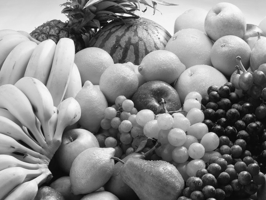
\includegraphics[scale=0.4]{original}} 
        \subfloat{\label{fig:post}
          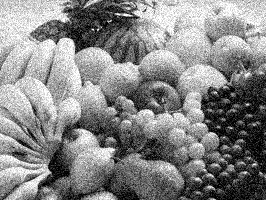
\includegraphics[scale=0.4]{noise}}                              
      \end{tabular}
      \caption{Left: Original gray-value image. Right: Image with added Gaussian noise $(\sigma=0.1)$.}
      \label{fig:original}
    \end{figure}

    \begin{figure}[!b]
      \centering
        \begin{tabular}{c}
        \subfloat{\label{fig:pre}
         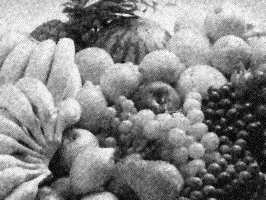
\includegraphics[scale=0.4]{t1}} 
        \subfloat{\label{fig:post}
          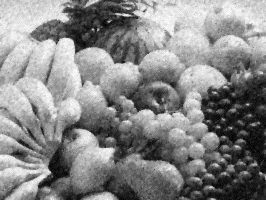
\includegraphics[scale=0.4]{t5}} \\
        \subfloat{\label{fig:ssdf}
          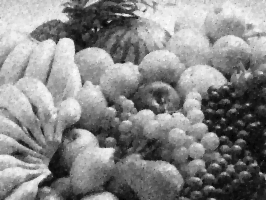
\includegraphics[scale=0.4]{t10}}  
        \subfloat{\label{fig:ssdf}
          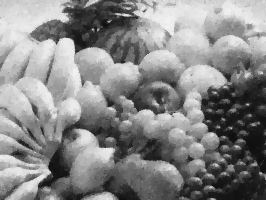
\includegraphics[scale=0.4]{t100}}                                               
        \subfloat{\label{fig:gt}
          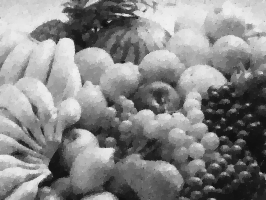
\includegraphics[scale=0.4]{tconverged}}                                
      \end{tabular}
      \caption{Estimated $\tilde{u}$ (gradient descent) for iterations $t=1$, $t=5$, $t=10$, $t=100$ and when convergence is achieved (from top left to bottom right image).}
      \label{fig:progression}
    \end{figure}
    
    \begin{figure}[!b]
      \centering
        \begin{tabular}{c}
        \subfloat{\label{fig:pre}
         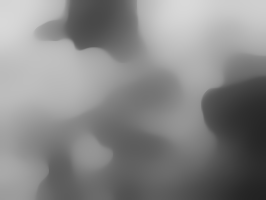
\includegraphics[scale=0.4]{lambda011000}} 
        \subfloat{\label{fig:post}
          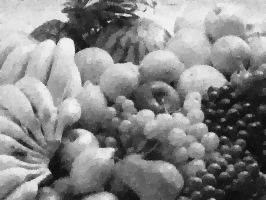
\includegraphics[scale=0.4]{lambda15}}
        \subfloat{\label{fig:post}
          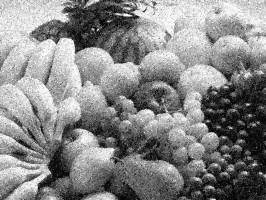
\includegraphics[scale=0.4]{lambda50}}                        
      \end{tabular}
      \caption{Left: $\lambda=0.1$. Middle: $\lambda=15$. Right: $\lambda=50$.}
      \label{fig:values}
    \end{figure}

Finally, we performed a gridsearch for different values (\begin{math}\left\{0,0.1,1,5,10,15,20,25,30,35,40\right\}\end{math}) of \begin{math}\lambda\end{math} to estimate the optimal value with respect to the error between the restored image \begin{math}\tilde{u}\end{math} and the ground truth image \begin{math}u\end{math}. The error was quantified via the sum of squared differences: \begin{math}SSD=\sum_{i}\sum_{j}\left(\tilde{u}(i,j)-u(i,j)\right)^{2}\end{math}. When we plot values for \begin{math}SSD\end{math} against \begin{math}\lambda\end{math} in figure \ref{fig:plot}, we can see that the optimal value for \begin{math}\lambda\end{math} corresponds to 15. All experiments have been performed with a maximum number of iterations \begin{math}T=1000\end{math} and backtracking line search parameters \begin{math}\alpha=0.05\end{math} and \begin{math}\beta=0.05\end{math} (empirically chosen).

    \begin{figure}[!h]
      \centering
         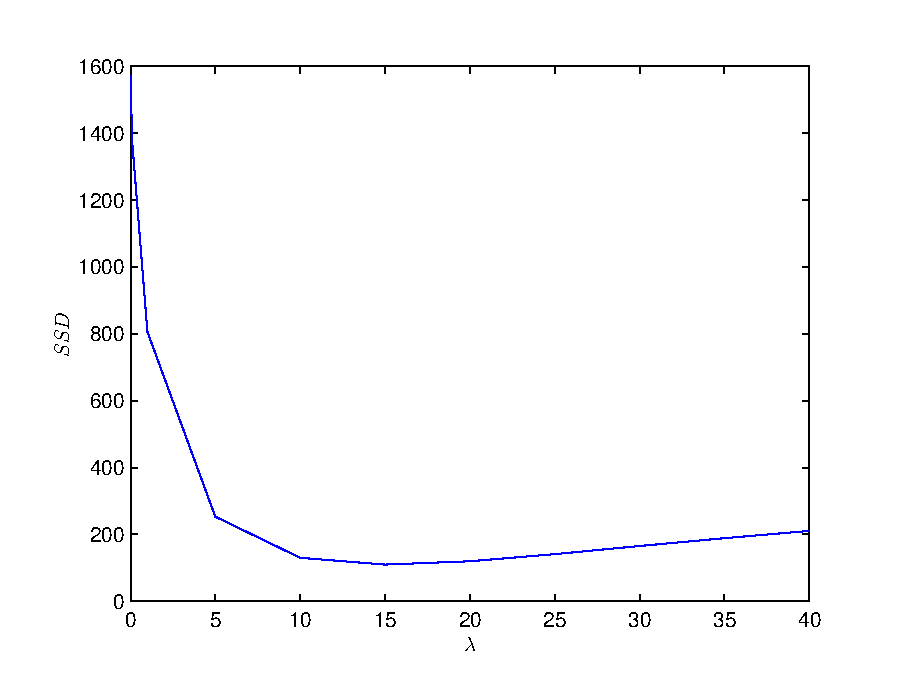
\includegraphics[scale=0.4]{lambdaplot.eps}                 
      \caption{Plot of $SSD$ vs. $\lambda$. Minima of $SSD=111.33$ for $\lambda=15$.}
      \label{fig:plot}
    \end{figure}
    
\subsection{Algorithm 2 -- Primal-Dual method}

We employed the same experimental setting to evaluate our primal-dual algorithm for solving the total variation image denoising problem. We chose \begin{math}\tau=0.02\end{math}, \begin{math}\sigma=\frac{0.95}{\left\|K\right\|^{2}\tau}\end{math} for all experiments (empirically chosen). In figure \ref{fig:progressionDual}, the progression of the denoising is shown for different iterations, starting with the initial estimate and ending with the image obtained at convergence. Note that the convergence of the primal-dual algorithm seems to be faster and for the present choice of parameters and convergence criterion is usually satisfied at around 70 iterations (compared to over 500 iterations for the gradient descent). This is also appearant when comparing the level of noise present in the image for each of the method for \begin{math}t=5\end{math}.

    \begin{figure}[!b]
      \centering
        \begin{tabular}{c}
        \subfloat{\label{fig:pre}
         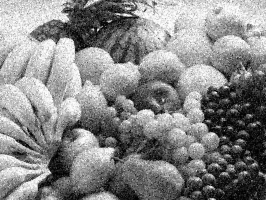
\includegraphics[scale=0.4]{t1d}} 
        \subfloat{\label{fig:post}
          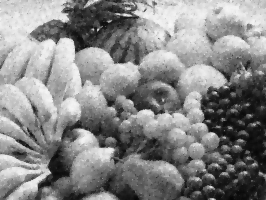
\includegraphics[scale=0.4]{t5d}} \\
        \subfloat{\label{fig:ssdf}
          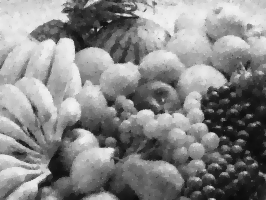
\includegraphics[scale=0.4]{t10d}}  
        \subfloat{\label{fig:ssdf}
          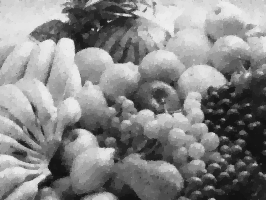
\includegraphics[scale=0.4]{t50d}}                                               
        \subfloat{\label{fig:gt}
          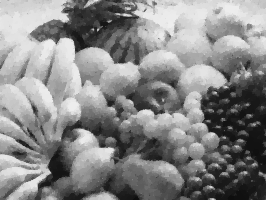
\includegraphics[scale=0.4]{tconvergedd}}                                
      \end{tabular}
      \caption{Estimated $\tilde{u}$ (primal-dual method) for iterations $t=1$, $t=5$, $t=10$, $t=50$ and when convergence is achieved (from top left to bottom right image).}
      \label{fig:progressionDual}
    \end{figure}
    
        \begin{figure}[!b]
      \centering
         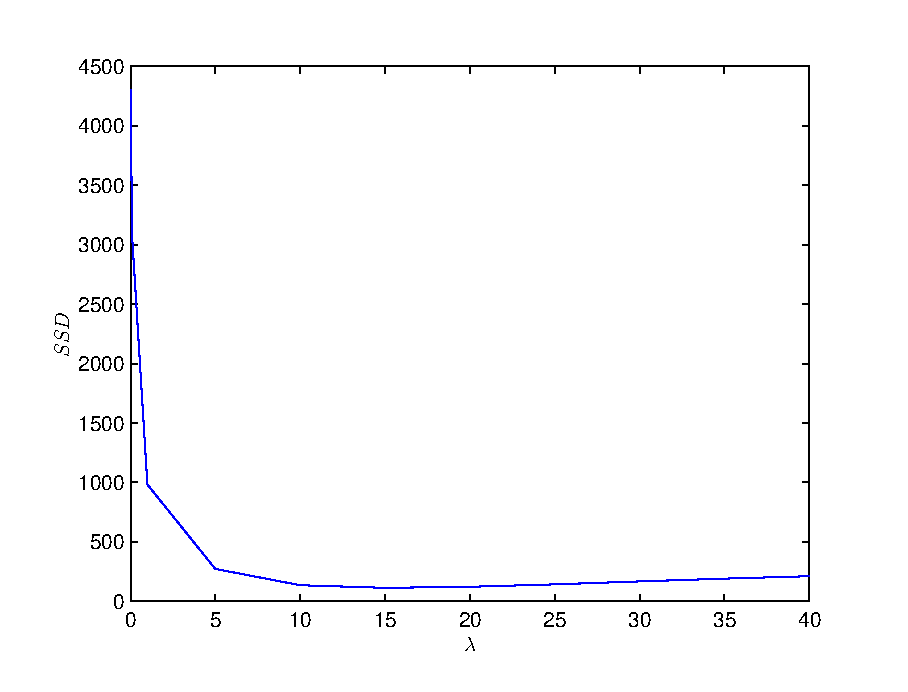
\includegraphics[scale=0.4]{optimalLambdaPrimalDual.eps}                 
      \caption{Plot of $SSD$ vs. $\lambda$. Minima of $SSD=112.75$ for $\lambda=15$.}
      \label{fig:plotDual}
    \end{figure}
    
Moreover, we also performed a gridsearch for the same range of values of \begin{math}\lambda\end{math} as before. When we plot values for \begin{math}SSD\end{math} against \begin{math}\lambda\end{math} in figure \ref{fig:plotDual}, we can see that the optimal value for \begin{math}\lambda\end{math} corresponds again to 15. All experiments have been performed with a maximum number of iterations \begin{math}T=1000\end{math}.


\section{Discussion}

From our results, we can clearly recognize that the proposed denoising method preserves edge information in the image. However, the method suffers from the introduction of staircase-artifacts. Extensions, such as e.g. Adaptive Total Variation regularization \cite{Chen2010}, have been proposed to resolve this problem. Furthermore, we can see that \begin{math}\lambda\end{math} is responsible for the trade-off between the least-squares penalty and total variation regularization. A very low \begin{math}\lambda\end{math} corresponds to a strong regularization. Thus, we downweight the correspondence between our estimate and the initial, noisy image. Moreover, we observed an increase in the number of iterations necessary to achieve convergence when \begin{math}\lambda\end{math} is small. A very high \begin{math}\lambda\end{math} corresponds to a weak regularization. In other words, we emphasize the importance of the correspondence between our estimate and the noisy image. When increasing \begin{math}\lambda\end{math}, starting from a low value, we observe a sharp decrease in \begin{math}SSD\end{math} with an optimum for intermediate values, followed by a gradual increase in error for large values.

When we compare algorithm 1 (gradient descent) with algorithm 2 (primal-dual method), we observe that regarding the \begin{math}SSD\end{math} both methods reach a comparable optimal value. Furthermore, the behavior of the \begin{math}SSD\end{math} and convergence with respect to \begin{math}\lambda\end{math} is for both algorithms the same (figure \ref{fig:plot} and \ref{fig:plotDual}). Consequently, we can state that both algorithms reach an equivalent solution. However, if we compare the algorithms with respect to computational time, we can see a distinct advantage for the primal-dual method, which converges in 0.75 seconds (averaged over 5 runs) compared to 31.87 seconds for the gradient descent (\begin{math}\lambda=15\end{math}).

In summary, the regularization parameter \begin{math}\lambda\end{math} has a strong influence on the final result and should be carefully chosen (i.e. optimized). The primal-dual algorithm shows superior computation time compared to the gradient descent method.

\appendixpage
\begin{appendices}
 \section{Derivation of $\nabla_{u}E(u)$}
 \label{appendixDer}
\begin{flushleft}
\begin{eqnarray}
   E(u) &=& \frac{\lambda}{2}LSQ(u,g) + TV(u)\nonumber \\
   %&=& (x^2+2)^2 -4x^2 \nonumber \\
   %\nonumber \\
   \Rightarrow (\nabla_{u}E(u))_{i,j} &=& \frac{\partial LSQ(u,g)}{\partial u[i,j]} + \frac{\partial TV(u)}{\partial u[i,j]} \nonumber \\
   %\nonumber \\
   \frac{\partial LSQ(u,g)}{\partial u[i,j]} &=& \lambda(u[i,j]-g[i,j]) \nonumber \\
   %\nonumber \\
   \frac{\partial TV(u)}{\partial u[i,j]} &=& \frac{\partial \tau[i,j]}{\partial u[i,j]} + \frac{\partial \tau[i-1,j]}{\partial u[i,j]} + \frac{\partial \tau[i,j-1]}{\partial u[i,j]} \nonumber \\
   %\nonumber \\
   \frac{\partial \tau[i,j]}{\partial u[i,j]} &=& \frac{\partial}{\partial u[i,j]}\sqrt{(u[i+1,j]-u[i,j])^2+(u[i,j+1]-u[i,j])^2} \nonumber \\
   &=& \frac{2u[i,j]-u[i+1,j]-u[i,j+1]}{\tau[i,j]} \nonumber \\
   \frac{\partial \tau[i-1,j]}{\partial u[i,j]} &=& \frac{\partial}{\partial u[i,j]}\sqrt{(u[i,j]-u[i-1,j])^2+(u[i-1,j+1]-u[i-1,j])^2} \nonumber \\
   &=& \frac{u[i,j]-u[i-1,j]}{\tau[i-1,j]} \nonumber \\
   \frac{\partial \tau[i,j-1]}{\partial u[i,j]} &=& \frac{\partial}{\partial u[i,j]}\sqrt{(u[i+1,j-1]-u[i,j-1])^2+(u[i,j]-u[i,j-1])^2} \nonumber \\
   &=& \frac{u[i,j]-u[i,j-1]}{\tau[i,j-1]} \nonumber \\
   %\nonumber \\
   \Rightarrow (\nabla_{u}E(u))_{i,j} &=& \lambda(u[i,j]-g[i,j]) + \frac{2u[i,j]-u[i+1,j]-u[i,j+1]}{\tau[i,j]} \nonumber \\
   && + \frac{u[i,j]-u[i-1,j]}{\tau[i-1,j]} + \frac{u[i,j]-u[i,j-1]}{\tau[i,j-1]} \nonumber
\end{eqnarray}
\end{flushleft}
 
 
 
\end{appendices}

\nocite{*}
\bibliography{COProject}

%progression

%very high low lambda, describe role of lambda. Bad convergence for low lambda

%optimal lambda

%edge-preserving but staircasing artifacts introduced. Use adaptive TV denoising to cope with those effects.

%\section*{Denoising}
%
%\begin{enumerate}
%\item \textbf{Problem.} Briefly describe the problem.
%\item \textbf{Motivations.} Describe the reasons and motivations behind this problem.
%\item \textbf{Derivation of gradient.} In this section you should:
%
%\begin{itemize}
%\item Write the finite difference approximation of the objective function $E$.
%\item Compute the gradient of the objective function $\nabla_uE$.  
%\end{itemize}
%
%
%\item \textbf{Implement gradient descent for denoising.} In this section you should:
%
%\begin{itemize}
%\item Show some images, as the the gradient method progresses iteration by iteration. Display the initial and the final image and 3 more images in between.
%\end{itemize}
%
%\item \textbf{Show images obtained by very high, very low and optimal $\lambda$.} In this section you should:
%
%\begin{itemize}
%\item Display 3 images with different $\lambda$ (very low, very high and optimal).
%\item Describe the effect of $\lambda$ on the solution.
%\end{itemize}
%
%\item \textbf{ Find optimal $\lambda$.} In this section you should:
%
%\begin{itemize}
%\item Display the $SSD$ vs. $\lambda$ graph.
%\item Describe the effect of $\lambda$ with respect to the $SSD$ between the ground truth and the solution image.
%\end{itemize}
%
%
%\end{enumerate}


 \end{document}
 
 